\section{Pilastro $P27$}\label{sec:p27}

Come raffigurato in figura~\ref{fig:pianoPrimo} di pagina~\pageref{fig:pianoPrimo} il pilastro $P27$ è un pilastro centrale di dimensione $30\times 30\,cm$. Il calcolo dell'area di influenza del pilastro verrà eseguito per ogni piano dell'edificio. Si anticipa che piano secondo e copertura hanno lo stesso schema statico e perciò la medesima area di influenza.

\subsection{Copertura}

\begin{figure}
	\centering
	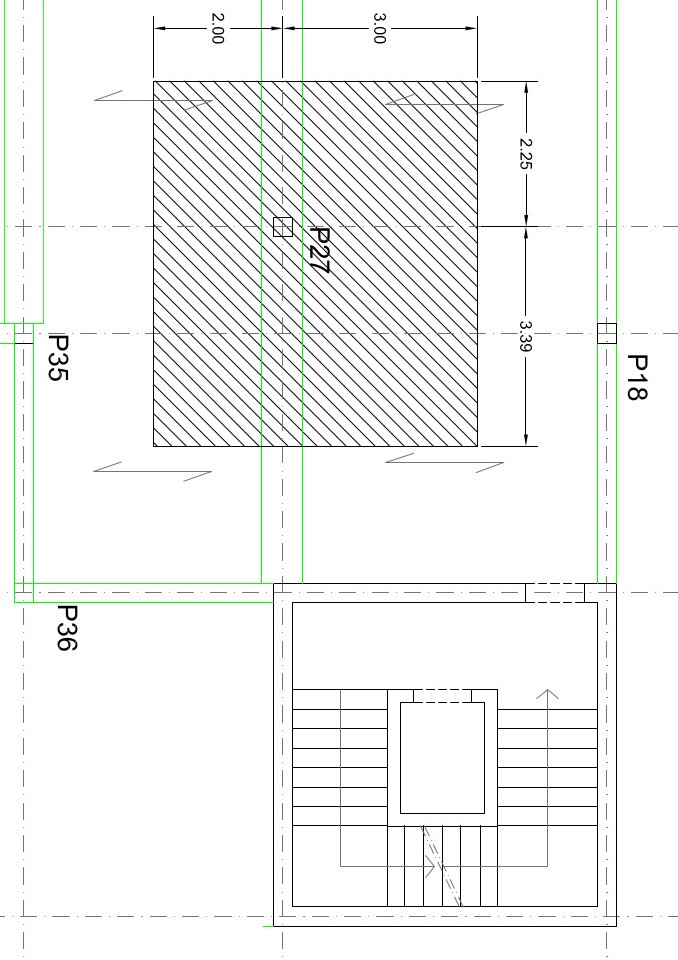
\includegraphics[height=.3\textheight]{p27_copertura}
	\caption{Area di influenza del pilastro $P27$ in copertura}
\end{figure}

